% !TEX TS-program = XeLaTeX
% use the following command:
% all document files must be coded in UTF-8
\documentclass[english]{textolivre}
% build HTML with: make4ht -e build.lua -c textolivre.cfg -x -u article "fn-in,svg,pic-align"

\journalname{Texto Livre}
\thevolume{18}
%\thenumber{1} % old template
\theyear{2025}
\receiveddate{\DTMdisplaydate{2025}{1}{27}{-1}} % YYYY MM DD
\accepteddate{\DTMdisplaydate{2025}{3}{3}{-1}}
\publisheddate{\DTMdisplaydate{2025}{7}{23}{-1}}
\corrauthor{Akhmad Habibi}
\articledoi{10.1590/1983-3652.2025.57135}
%\articleid{NNNN} % if the article ID is not the last 5 numbers of its DOI, provide it using \articleid{} commmand 
% list of available sesscions in the journal: articles, dossier, reports, essays, reviews, interviews, editorial
\articlesessionname{dossier}
\runningauthor{Firdaus et al.} 
%\editorname{Leonardo Araújo} % old template
\sectioneditorname{Hugo Heredia Ponce}
\layouteditorname{Leonado Araújo}

\title{Factors affecting Indonesian pre-service EFL teachers’ AI acceptance and use}
\othertitle{Fatores que afetam a aceitação e o uso da IA por parte dos futuros professores de inglês como língua estrangeira da Indonésia}
% if there is a third language title, add here:
%\othertitle{Artikelvorlage zur Einreichung beim Texto Livre Journal}

\author[1]{Rangga Firdaus~\orcid{0000-0003-4139-9946}\thanks{Email: \href{mailto:ranggafirdaus@fkip.unila.ac.id}{ranggafirdaus@fkip.unila.ac.id}}}
\author[2,3]{Akhmad Habibi~\orcid{0000-0001-7687-2858}\thanks{Email: \href{mailto:akhmadhabibi@korea.ac.kr}{akhmadhabibi@korea.ac.kr}}}
\author[3]{Robi Hendra~\orcid{0000-0002-2471-3107}\thanks{Email: \href{mailto:robi.hendra@unja.ac.id}{robi.hendra@unja.ac.id}}}
\author[4]{Mohd Sofian Omar Fauzee~\orcid{0000-0002-6841-9647}\thanks{Email: \href{mailto:sofian.fauzees@newinti.edu.my}{sofian.fauzees@newinti.edu.my}}}
\author[1]{Sheren Dwi Oktaria~\orcid{0000-0002-7075-5762}\thanks{Email: \href{mailto:sheren.dwi@fkip.unila.ac.id}{sheren.dwi@fkip.unila.ac.id}}}
\author[3]{Muhammad Sofwan~\orcid{0000-0001-6936-1267}\thanks{Email: \href{mailto:muhammad.sofwan@unja.ac.id}{muhammad.sofwan@unja.ac.id}}}
\author[5]{Turki Mesfer Alqahtani~\orcid{0000-0002-7226-9602}\thanks{Email: \href{mailto:turki.mf.h@gmail.com}{turki.mf.h@gmail.com}}}
\affil[1]{Universitas Lampung, Program Studi Magister Teknologi Pendidikan, FKIP, Indonesia.}
\affil[2]{Korea University, Graduate School of Education, Seoul, Republic of Korea.}
\affil[3]{Universitas Jambi, Fakultas Keguruan dan Ilmu Pendidikan, Jambi, Indonesia.}
\affil[4]{INTI International University, Faculty of Education and Liberal Arts, Nilai, Malaysia.}
\affil[5]{Jazan University, College of Arts and Humanities, e-Learning Centre and Department of Educational Sciences, Jazan, Saudi Arabia.}

\addbibresource{article.bib}
% use biber instead of bibtex
% $ biber article

% used to create dummy text for the template file
\definecolor{dark-gray}{gray}{0.35} % color used to display dummy texts
\usepackage{lipsum}
\SetLipsumParListSurrounders{\colorlet{oldcolor}{.}\color{dark-gray}}{\color{oldcolor}}

% used here only to provide the XeLaTeX and BibTeX logos
\usepackage{hologo}

% if you use multirows in a table, include the multirow package
\usepackage{multirow}

% provides sidewaysfigure environment
\usepackage{rotating}

% CUSTOM EPIGRAPH - BEGIN 
%%% https://tex.stackexchange.com/questions/193178/specific-epigraph-style
\usepackage{epigraph}
\renewcommand\textflush{flushright}
\makeatletter
\newlength\epitextskip
\pretocmd{\@epitext}{\em}{}{}
\apptocmd{\@epitext}{\em}{}{}
\patchcmd{\epigraph}{\@epitext{#1}\\}{\@epitext{#1}\\[\epitextskip]}{}{}
\makeatother
\setlength\epigraphrule{0pt}
\setlength\epitextskip{0.5ex}
\setlength\epigraphwidth{.7\textwidth}
% CUSTOM EPIGRAPH - END

% to use IPA symbols in unicode add
%\usepackage{fontspec}
%\newfontfamily\ipafont{CMU Serif}
%\newcommand{\ipa}[1]{{\ipafont #1}}
% and in the text you may use the \ipa{...} command passing the symbols in unicode

% LANGUAGE - BEGIN
% ARABIC
% for languages that use special fonts, you must provide the typeface that will be used
% \setotherlanguage{arabic}
% \newfontfamily\arabicfont[Script=Arabic]{Amiri}
% \newfontfamily\arabicfontsf[Script=Arabic]{Amiri}
% \newfontfamily\arabicfonttt[Script=Arabic]{Amiri}
%
% in the article, to add arabic text use: \textlang{arabic}{ ... }
%
% RUSSIAN
% for russian text we also need to define fonts with support for Cyrillic script
% \usepackage{fontspec}
% \setotherlanguage{russian}
% \newfontfamily\cyrillicfont{Times New Roman}
% \newfontfamily\cyrillicfontsf{Times New Roman}[Script=Cyrillic]
% \newfontfamily\cyrillicfonttt{Times New Roman}[Script=Cyrillic]
%
% in the text use \begin{russian} ... \end{russian}
% LANGUAGE - END

% EMOJIS - BEGIN
% to use emoticons in your manuscript
% https://stackoverflow.com/questions/190145/how-to-insert-emoticons-in-latex/57076064
% using font Symbola, which has full support
% the font may be downloaded at:
% https://dn-works.com/ufas/
% add to preamble:
% \newfontfamily\Symbola{Symbola}
% in the text use:
% {\Symbola }
% EMOJIS - END

% LABEL REFERENCE TO DESCRIPTIVE LIST - BEGIN
% reference itens in a descriptive list using their labels instead of numbers
% insert the code below in the preambule:
%\makeatletter
%\let\orgdescriptionlabel\descriptionlabel
%\renewcommand*{\descriptionlabel}[1]{%
%  \let\orglabel\label
%  \let\label\@gobble
%  \phantomsection
%  \edef\@currentlabel{#1\unskip}%
%  \let\label\orglabel
%  \orgdescriptionlabel{#1}%
%}
%\makeatother
%
% in your document, use as illustraded here:
%\begin{description}
%  \item[first\label{itm1}] this is only an example;
%  % ...  add more items
%\end{description}
% LABEL REFERENCE TO DESCRIPTIVE LIST - END


% add line numbers for submission
%\usepackage{lineno}
%\linenumbers

\begin{document}
\maketitle

\begin{polyabstract}
\begin{abstract}
Integrating artificial intelligence in language education, particularly for pre-service English as a Foreign Language (EFL) teachers, presents unique challenges and opportunities. This research seeks to extend the technology acceptance model (TAM) by integrating technological pedagogical and content knowledge (TPACK) to predict behavioral intentions and actual use of AI technologies in an EFL context. Employing partial least squares structural equation modeling, the sample consisted of 436 pre-service EFL teachers. The findings showed that perceived ease of use impacts perceived usefulness ($\beta$=0.674) and attitudes ($\beta$=0.387). Perceived usefulness affects attitudes ($\beta$=0.452) and AI-behavioral intention ($\beta$=0.216). The attitudes variable influences AI-behavioral intention ($\beta$=0.206). Technological content and technological pedagogical knowledge contribute to TPACK ($\beta$=0.278, $\beta$=0.311). TPACK impacts AI-behavioral intention ($\beta$=0.350) and AI-use ($\beta$=0.557). By extending the TAM with TPACK, this study offers insights into optimizing AI adoption among future language educators, thereby fostering innovative teaching practices that enhance language learning experiences for students. The current study covers two areas of Sustainable Development Goals (SDGs): Higher education quality in the EFL area (SDG 4 - Quality Education) and digital transformation in education (SDG 17 – Partnerships for the Goals).

\keywords{Artificial Intelligence \sep Pre-service EFL teacher \sep Survey \sep TAM \sep TPACK}
\end{abstract}

\begin{portuguese}
\begin{abstract}
A integração da inteligência artificial no ensino de idiomas, particularmente para futuros professores de inglês como língua estrangeira (EFL), apresenta desafios e oportunidades únicos. Esta pesquisa busca estender o modelo de aceitação de tecnologia (TAM) integrando o conhecimento pedagógico tecnológico e o conhecimento de conteúdo (TPACK) para prever intenções comportamentais e o uso real de tecnologias de IA em um contexto de EFL. Empregando modelagem de equações estruturais de mínimos quadrados parciais, a amostra consistiu de 436 futuros professores de EFL. Os resultados mostraram que a facilidade de uso percebida impacta a utilidade percebida ($\beta$ = 0,674) e as atitudes ($\beta$ = 0,387). A utilidade percebida afeta as atitudes ($\beta$ = 0,452) e a intenção comportamental da IA ($\beta$ = 0,216). A variável atitudes influencia a intenção comportamental da IA ($\beta$ = 0,206). O conteúdo tecnológico e o conhecimento pedagógico tecnológico contribuem para o TPACK ($\beta$ = 0,278, $\beta$ = 0,311). O TPACK impacta a intenção comportamental da IA ($\beta$ = 0,350) e o uso da IA ($\beta$ = 0,557). Ao estender o TAM com o TPACK, este estudo oferece \textit{insights} sobre como otimizar a adoção da IA entre futuros educadores de línguas, promovendo práticas de ensino inovadoras que aprimoram as experiências de aprendizagem de línguas para os alunos. O estudo atual abrange duas áreas dos Objetivos de Desenvolvimento Sustentável (ODS): qualidade do ensino superior na área de inglês como língua estrangeira (ODS 4 - Educação de Qualidade) e transformação digital na educação (ODS 17 - Parcerias para os Objetivos).

\keywords{Inteligência Artificial \sep Professor de inglês em formação inicial \sep Pesquisa \sep TAM \sep TPACK}
\end{abstract}
\end{portuguese}
% if there is another abstract, insert it here using the same scheme
\end{polyabstract}

\section{Introduction}\label{sec-intro}
Artificial intelligence (AI) in teaching English as a foreign language (EFL) stands out as a frontier and pivot for innovation when technology is constantly changing \cite{darwin2024critical}. Therefore, training pre-service EFL teachers to become familiar with AI technologies and their use to improve language acquisition becomes essential.  Prior studies have explored AI use in education through frameworks such as UTAUT, IS Success model, TAM, and TPACK \cite{ma2024tam,venkatesh2022utaut,yoon2023aispeakers}. The current research elaborates on how pre-service EFL teachers perceived AI in their teaching practicum. The broad applicability of traditional models like TAM, which combine perceived usefulness (PU), perceived ease of use (PEOU), and attitudes (ATT) to forecast AI-behavioral intention (AI-BI) and AI-use (AI-USE), is frequently criticized for lacking specific contextual nuances. A more specialized method of comprehending AI acceptance and use in the unique setting of language education is provided by this study’s integration TAM with TPACK (technological pedagogical and content knowledge). TPACK highlights the interaction between knowledge of technology, pedagogy, and content. This study incorporates the TPACK framework, including technological pedagogical knowledge (TPK) and technological content knowledge (TCK), as the variables examined are grounded in technology-related knowledge domains.

The intersection of the proposed hypotheses is crucial because teaching languages includes developing linguistic information as well as cultural and communicative skills \cite{aladwan2024useintention}. The current study may assist in establishing professional development programs that better reflect pre-service EFL teachers’ needs. The programs could lead to more creative English teaching approaches and increased classroom technology adoption. To prepare students for 21st-century education, policymakers need to understand how future teachers will respond to advanced AI tools, like language learning apps and AI feedback systems. Given the phenomenon, this study elaborated on Indonesian pre-service EFL teachers’ AI-BI and AI-USE during teaching practicum. Thus, this research sits at the intersection of acceptance, pedagogy, technology, and language instruction to contribute to the development of Indonesian higher education. To meet the objectives of the research, 11 hypotheses were proposed within this study context, detailed in the literature review section (\Cref{fig1}).

\section{Literature review}\label{sec-normas}
Understanding how teachers use technology is vital in the fast-changing world of educational technology. The current study proposes a new paradigm that combines TAM with the TPACK frameworks to better comprehend AI acceptance and use for pre-service EFL teachers \cite{aladwan2024useintention,habibi2023mlms}. \Cref{fig1} shows how these two models are integrated in the suggested paradigm. PEOU, PU, and ATT are the main elements of the TAM, which was established to explain user acceptance. PEOU is the degree to which a person believes a system will be easy to use, whereas PU is the degree to which it will improve their work performance. Our model represents these two notions, which lead to attitudes towards using technology, pre-service EFL teachers’ positive or negative feelings about using a particular technology \cite{davis1989tam}. TPACK framework organizes how teachers’ technology, pedagogy, and content knowledge improve learning \cite{mishra2009tpack}. The concept used in this study covers three factors, TCK, TPK, and TPACK, to influence AI acceptance and use in the EFL field. The model includes AI-BI, influenced by PU, ATT, TCK, TPK and TPACK components, underlining AI’s importance in current education and AI-USE, which is expected to be influenced by AI-BI and TPACK. Prior studies have combined TAM and TPACK in their studies, reporting the significance of supporting variables to understand the use and acceptance of technology with TPACK during instructional activities, such as virtual reality in education \cite{thohir2023vr}, technology \cite{cheng2024tpack}, and AI \cite{sun2024ai}.

\subsection{Perceived ease of use (PEOU)}\label{sec-conduta}
We emphasize the importance of creating AI tools that are not only strong in function but also user-friendly and accessible, particularly for pre-service EFL teachers \cite{davis1989tam}. In this study, PEOU is hypothesized to influence PU directly. Fundamental to TAM, the idea that PEOU influences PU has been extensively researched in several educational situations, including language teaching and learning and in a study with pre-service teachers, including those with an EFL concentration \cite{allali2024chatgpt,dehghani2024chatgpt,liu2023chatgpt,ma2024tam,wu2023aiuse,zou2023speechai}. \textcite{wu2023aiuse} discovered that EFL learners were more inclined to view AI technologies as beneficial for learning when they were thought to be simple to use and navigate. In Iran \cite{dehghani2024chatgpt}, it was revealed that EFL teachers’ PEOU and PU were significantly correlated in the context of ChatGPT use in English teaching. PEOU influences ATT (positive or negative feelings about AI use in EFL teaching practicum) toward AI use in teaching practicum. Some prior studies have explored this relationship in technology adoption in education \cite{alabdullatif2023chatbots,chen2024mr,ma2024tam,wu2023aiuse,yuviler2024chatbot}. \textcite{wu2023aiuse} through a mixed method study investigated the relationship between PEOU and ATT about AI in the setting of pre-service EFL learners. They observed that EFL learners’ opinions toward AI tools improved when they perceived them as less intimidating and more uncomplicated to include in their learning tools. The observation is fundamental in language education, where language learning and teaching complexity may first make learners nervous about implementing new technology in learning \cite{wu2023aiuse}. The findings might be promising, increasing the desire to learn and apply AI, creating an atmosphere that permits and promotes innovation in language teaching and learning. However, several studies disclosed the insignificant relationship between PEOU and ATT \cite{alabdullatif2023chatbots,chen2024mr,yuviler2024chatbot}, suggesting the relationship still needs to be examined in several contexts and settings. Two hypotheses were established regarding the roles of PEOU towards PU and ATT. 

\begin{description}
    \item[H1]: PEOU significantly influences PU
    \item[H2]: PEOU significantly influences ATT
\end{description}

\subsection{Perceived usefulness (PU)}\label{sec-fmt-manuscrito}
PU (the degree to which AI will improve their teaching performance) and how these affect ATT and AI-BI in pre-service EFL teachers, in particular, drive the incorporation of AI in the classroom. This study examines two crucial theories investigating these dynamics derived from the TAM \cite{davis1989tam}. Prior studies revealed that PU is a key component of technology adoption, which directly impacts ATT toward the technology \cite{gumbi2024dgb,peng2022kiosks,wang2021aiadoption,weng2018tam}. \textcite{gumbi2024dgb} who studied pre-service teachers, including those in EFL, revealed that views toward AI tools improve when perceived as helpful for improving student learning outcomes or teaching. However, \textcite{wang2021aiadoption} disclosed the insignificant relationship between PU and ATT among Chinese teachers on the use of AI in education. PU in this study is also expected to significantly correlate with AI-BI. Pre-service EFL teachers’ intention to integrate AI into their teaching practices increases with their perception of the value of technology in accomplishing learning objectives \cite{alabdullatif2023chatbots,dehghani2024chatgpt,yao2024intention,zhang2023acceptance}. The correlation suggests that for AI to be successfully included in EFL instruction, it needs to be perceived as directly advancing the learning goals, which will increase motivation to use AI in teaching \cite{yao2024intention,zhang2023acceptance}. The two hypotheses show that pre-service EFL teachers’ ATT toward AI is influenced, which also strongly influences their desire to include these technologies in their instruction. The elaboration implies that pre-service teacher education programs should emphasize showcasing AI’s valuable applications to foster favorable views and intentions regarding its application in classroom environments.

\begin{description}
    \item[H3]: PU has a significant influence on ATT.
    \item[H4]: PU significantly influences AI-BI.
\end{description}



\subsection{Attitudes (ATT)}\label{sec-formato}
Since ATT can substantially affect how AI is incorporated into future teaching practices, this link is particularly relevant for pre-service EFL teachers. In TAM, ATT frequently serves as the link between perception and action. Prior studies have also revealed the relationship between ATT and behavioral intention to use technology \cite{allali2024chatgpt,dehghani2024chatgpt,gumbi2024dgb,liu2023chatgpt,ma2024tam,weng2018tam,wu2023aiuse,zou2023speechai}. Teachers with favorable opinions of AI were likelier to implement these tools in their classes \cite{gumbi2024dgb}. Positivity toward AI suggests a willingness to investigate, test, and eventually incorporate new technologies into instructional strategies. One hypothesis was proposed to meet the study's objectives of revealing the correlation between ATT and AI-BI.

\begin{description}
    \item[H5]: ATT has a positive and significant correlation with AI-BI
\end{description}



\subsection{Technological content knowledge (TCK)}\label{sec-modelo}
TCK in this study refers to pre-service EFL teachers’ understanding of how technology can be used in conjunction with particular subject areas. It is hypothesized that TCK significantly influences pre-service EFL teachers’ AI-BI; some prior studies have supported a similar hypothesis \cite{an2023ai,habibi2020tpack,mailizar2021tpack,sofyan2023tpack}. In a study within the context of English teachers of middle schools in China, \textcite{an2023ai} elaborate that teachers are more likely to prepare for using AI when they comprehend how it may interact with language teaching materials. Comprehending how AI enhances content delivery influences teachers’ preparedness to integrate these technologies into their curriculum, as language education is content-rich \cite{habibi2020tpack}. Further, TCK is a key component of TPACK, which combines content knowledge and technology into a coherent teaching framework. Prior studies have explored the correlations \cite{an2023ai,habibi2020tpack,mailizar2021tpack,mansour2024stem,sofyan2023tpack}. For example, \textcite{habibi2020tpack} state that pre-service language teachers’ TCK development directly impacts pre-service teachers’ overall TPACK. Understanding how technology interacts with language teaching content (TCK) is essential for EFL teachers to advance their understanding of how to use technology to teach that content (TPACK) \cite{an2023ai}. The advancement is necessary because language instruction necessitates a sophisticated strategy in which technology complements the teaching methodology and improves the acquisition of linguistic and cultural components. Two hypotheses were proposed to examine TCK’s relationship with AI-BI and TPACK. 

\begin{description}
    \item[H6]: TCK significantly influences AI-BI.
    \item[H7]: TCK positively and significantly affects TPACK.
\end{description}


\subsection{Technological pedagogical knowledge (TPK)}\label{sec-organizacao}
TPK entails comprehending how technology can be used to improve or alter instructional practices, improving the intention to use technology \cite{voogt2010tpack}. Pre-service teachers’ intention to include AI in their teaching practices dramatically increases when they fully understand TPK \cite{an2023ai,habibi2020tpack,mailizar2021tpack,sofyan2023tpack}. Teachers are more inclined to embrace new technologies when they understand how AI can be pedagogically integrated to enhance language teaching techniques, such as through tailored learning paths, real-time pronunciation correction, or interactive speaking exercises  \cite{an2023ai,habibi2020tpack}. In addition, TPK is essential to the TPACK framework. TPK directly aids in developing TPACK for pre-service teachers, particularly those in EFL. Knowledge of what to teach (content) and how to utilize technology to teach that material is enhanced and complemented by an understanding of how to teach with technology or TPACK \cite{an2023ai,habibi2020tpack,mailizar2021tpack,sofyan2023tpack}. This process requires understanding how AI can be integrated into language instruction to accommodate various learning preferences, linguistic proficiency, and cultural quirks for EFL teachers. Pre-service teachers are able to recognize the comprehensive integration of technology in education, which is a defining characteristic of TPACK, as their TPK grows. We proposed two hypotheses regarding the role of TPK toward AI-BI and TPACK.

\begin{description}
    \item[H8]: TPK significantly affects AI-BI.
    \item[H9]: TPK significantly influences TPACK.
\end{description}


\subsection{Technological pedagogical and content knowledge (TPACK)}\label{sec-organizacao-latex}
TPACK thoroughly describes how technology can improve instruction by combining pedagogy, content knowledge, and technology. Pre-service teachers—including those with an EFL concentration—were more likely to indicate plans to include AI in their instruction if they had higher TPACK activities \cite{an2023ai,habibi2020tpack,mailizar2021tpack,sofyan2023tpack}. Pre-service teachers’ AI-BI toward implementing these technologies rise when they see how AI can be smoothly incorporated into lesson lesson planning, delivering materials, and assessing students \cite{an2023ai,mailizar2021tpack}. To ensure that future educators view AI as an essential component of their teaching toolkit rather than an add-on, this hypothesis emphasizes the necessity for educational programs to cultivate a thorough grasp of TPACK. Further, effective TPACK significantly improves the actual application of AI in education, as expected from the results of the data analysis. Pre-service EFL teachers can put their intentions into practice by learning how to use AI in their teaching strategies, adjusting to the needs of several students, and coordinating technology use with curriculum objectives \cite{an2023ai,habibi2020tpack,mailizar2021tpack,sofyan2023tpack}. Teachers who have mastered TPACK are more inventive when creating AI-infused lessons and more adept at resolving issues and adjusting to changing circumstances in the classroom \cite{an2023ai,habibi2020tpack,mailizar2021tpack}. The quality of language instruction is immediately impacted when AI is used for tailored learning paths, language analysis, or cultural immersion experiences, for example, as it becomes more practical and efficient.

\begin{description}
    \item[H10]: TPACK has a positive and significant impact on AI-BI.
    \item[H11]: TPACK significantly influences AI-USE.
\end{description}


\subsection{AI-behavioral intention (AI-BI)}\label{sec-titulo}
Within the framework of technology acceptance models, notably in educational settings, the connection between intention and actual use has been thoroughly investigated \cite{lavidas2024ai,strzelecki2024chatgpt,xiaohong2024intentions}. \textcite{strzelecki2024chatgpt} who studied the use of ChatGPT in students’ learning in higher education disclosed a close correlation between the actual use of AI in learning and a firm intention to employ it. The study implies that for students, when there is a strong desire to use AI—possibly because of the perceived advantages of improving tasks—this desire is likely to materialize in real-world applications such as the use of AI for interactive learning, including language learning and teaching as the context of the current study. A hypothesis was established to reveal the correlation between AI-BI and AI-USE in this study.

\begin{description}
    \item[H12]: AI-BI significantly affects AI-USE.
\end{description}


\begin{figure}[h!]
    \centering
    \begin{minipage}{0.75\linewidth}
    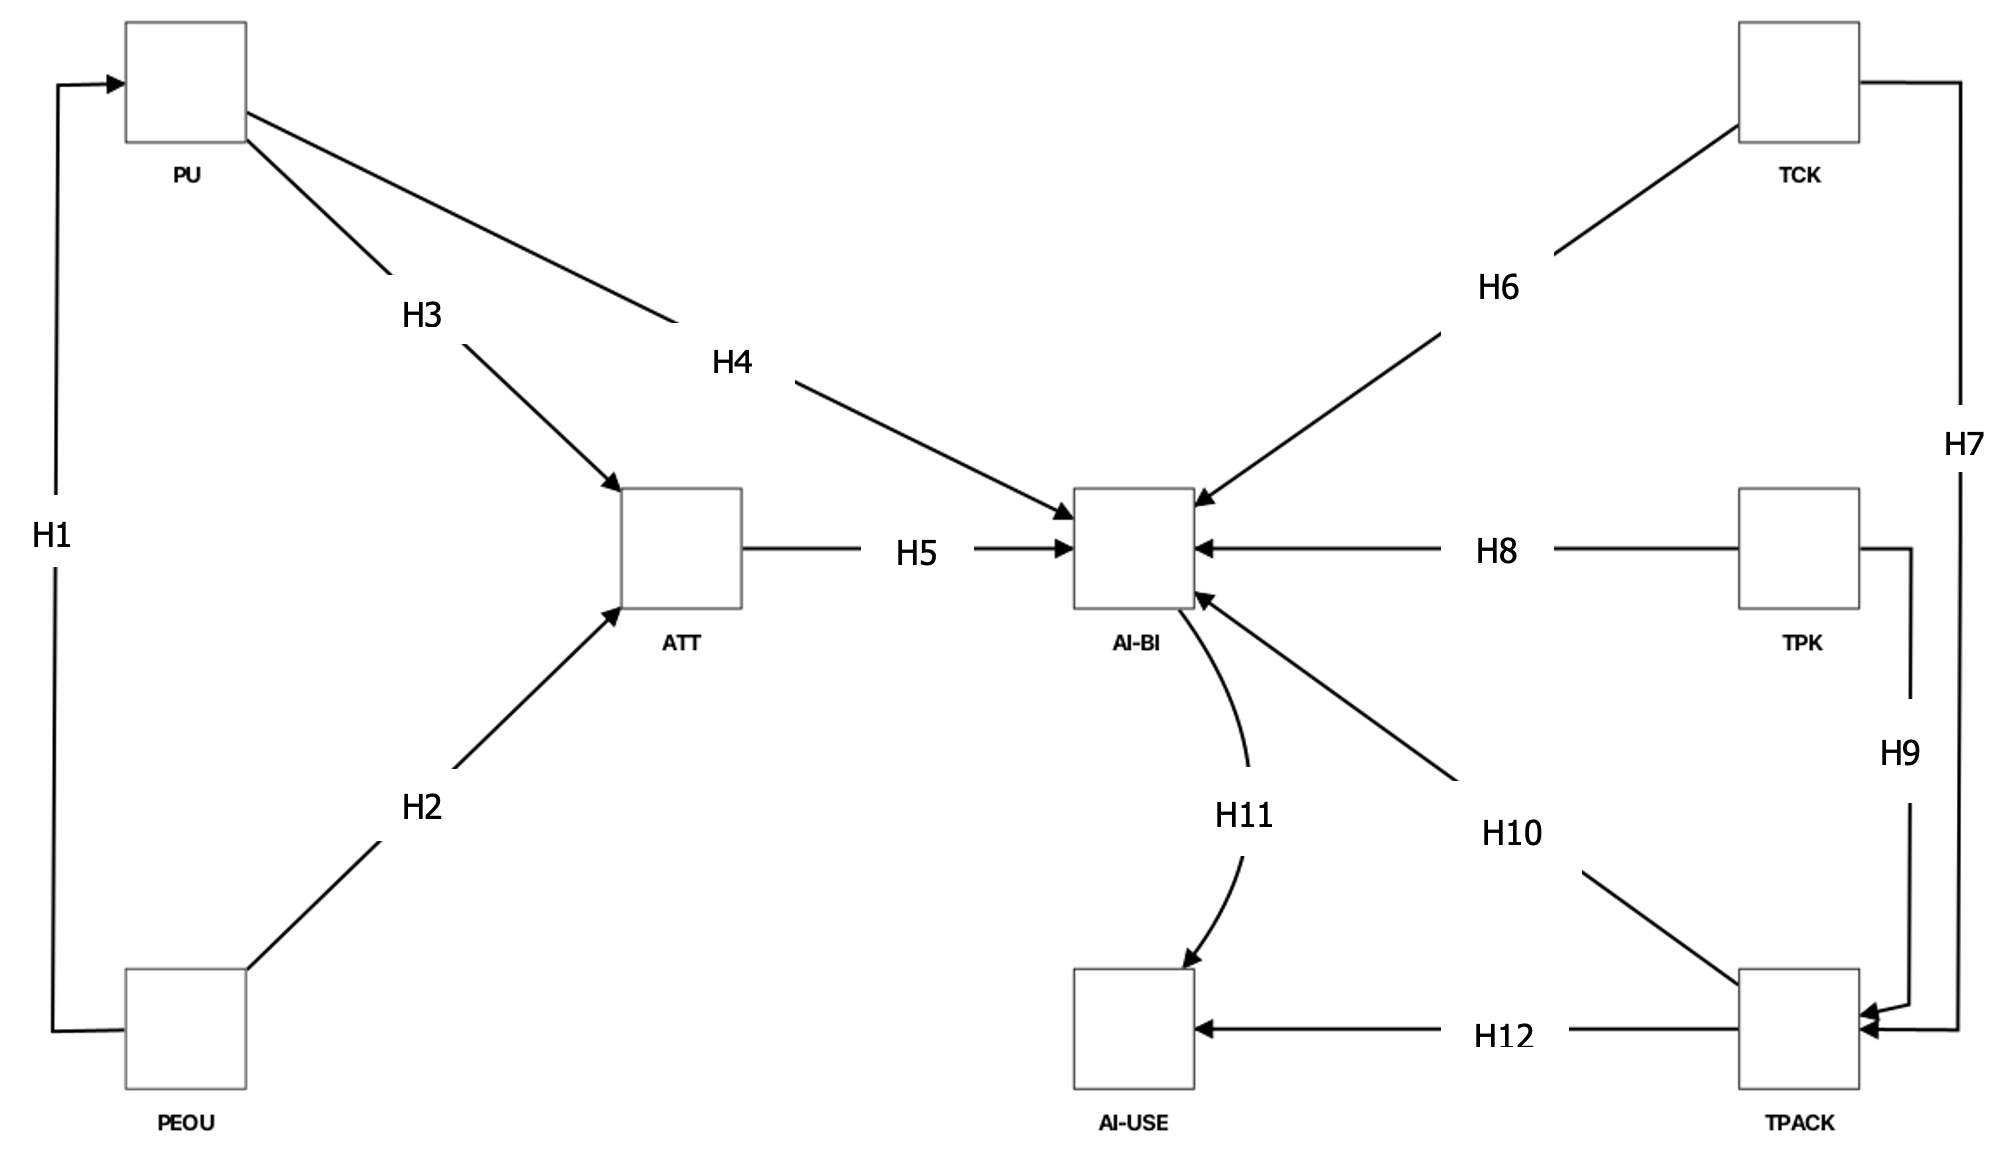
\includegraphics[width=\linewidth]{Fig1.png}
    \caption{Proposed model}
    \label{fig1}
    \source{The authors.}
    \notes{Perceived ease of use (PEOU),  perceived usefulness (PU), attitudes (ATT), technological content knowledge (TCK), technological pedagogical knowledge (TCK), technological pedagogical content knowledge (TCK),  artificial intelligence behavioral intention (AI-BI), artificial intelligence use (AI-USE).}
    \end{minipage}
\end{figure}

\section{Method}\label{sec-autores}
The current research was conducted through a quantitative approach with a survey as a data collection tool. The survey was selected to gain data that provide a more standardized and consistent evaluation that can be more easily combined and analyzed. This research was conducted from September 2024 to January 2025 using surveys as the data collection method \cite{ball2019survey,evans2005value}. A review of prior research and an evaluation of the validity and reliability of the instruments were conducted. The model was assessed using partial least squares structural equation modeling (PLS-SEM) \cite{cepeda2024plssem,habibi2024access,vaithilingam2024robustness}. The current investigation employed a predictive methodology to ascertain the causality model, as the study’s process is unaffected by assumptions on the distribution of data \cite{habibi2024utaut}. To improve the openness of the study for future replicability, the instrument and samples of the responses can be accessed in Figshare (\url{https://doi.org/10.6084/m9.figshare.28560584}).

\subsection{Instrumentation}\label{sec-idioma}
The literature review assists a researcher in defining the ideas and concepts within the theoretical framework and identifying suitable methodologies and instruments to achieve the research objectives. We modified and developed survey instruments based on prior related research (50 survey items); TAM \cite{aladwan2024useintention,wang2022tam2} and TPACK \cite{aladwan2024useintention,habibi2020tpack,mishra2009tpack}. Subsequently, the instruments were evaluated for face and content validity via interviews and the content validity index (CVI) to account for social, cultural, and contextual variations \cite{oliveira2022insulin}. A panel of six individuals, comprising four pre-service EFL teachers, one program staff members, and one teacher educator, discussed the adapted instruments to assess face validity. 

To establish content validity, we consulted five Indonesian experts regarding the instruments. The experts were academics in the domains of educational technology; some items were amended and five items were discarded due to their inapplicability in the academic setting of Indonesia, yielding a total of 45 items for the validation process. The characteristics of the items were evaluated using a 4-point scale (1 = not relevant/not clear/not simple to 4 = extremely relevant, very clear, very simple) by ten experts \cite{habibi2020tpack}. The Content Validity Index (CVI) was evaluated at both the item level (I-CVI) and the scale level (S-CVI) for the qualities of the three instruments. The CVI was calculated by assigning a score of 3 or 4 to the experts, then divided by the total number of experts. A score of 3 or 4 in the CVI theory a score of 3 or 4 is considered an affirmative response in CVI theory. The I-CVI must be no less than 0.780 with ten experts \cite{oliveira2022insulin}. In the computation of the S-CVI, the mean proportion of items on a single scale scored 3 or 4 (average agreement by experts = S-CVI/AVE). The cutoff value is 0.800, and most item values exceed 0.780 for I-CVI and 0.800 for S-CVI. 


\subsection{Data collection}\label{sec-resumo}
After completing face, content validity, and CVI assessments, we shared the instruments with the respondents \cite{rimando2015challenges}. The data were acquired from three Indonesian institutions with education faculties. The data distribution was conducted online using Google Forms. We spent three months collecting the data. all responses were compiled and processed using Microsoft Excel and SPSS. This study’s target population comprises all Indonesian pre-service EFL teachers in three institutions or universities. Utilizing stratified sampling, we segmented the target samples based on their universities. In this study, 436 respondents participated in the survey; 22.94\% of the respondents were men and 77.06\% were women. Universities A, B, and C accounted for 48.40\%, 33.72\%, and 17.89\%. In the first two semesters, the distribution was 0\%; in the third and fourth, 58.94\%, and in the fifth and higher, 41.06\%. 46.33\% of respondents were from cities, and 53.67\% were from urban areas. \Cref{tbl1} exhibits all details of the demographic information included in this study.

\begin{table}[h!]
\centering
\begin{threeparttable}
\caption{Demography of the respondents.}
\label{tbl1}
\begin{tabular}{lrr}
\toprule
Category & n. 436 & \% \\
\midrule
Gender & & \\
\quad Male & 100 & 22.94 \\
\quad Female & 336 & 77.06 \\
Institution & & \\
\quad University A & 211 & 48.40 \\
\quad University B & 147 & 33.72 \\
\quad University C & 78 & 17.89 \\
Semester & & \\
\quad 1\textsuperscript{st}-2\textsuperscript{nd} & 0 & 0 \\
\quad 3\textsuperscript{rd}-4\textsuperscript{th} & 257 & 58.94 \\
\quad 5\textsuperscript{th}-above & 179 & 41.06 \\
School location & & \\
\quad Urban & 234 & 53.67 \\
\quad City & 202 & 46.33 \\
\bottomrule
\end{tabular}
\source{The authors.}
\end{threeparttable}
\end{table}



\subsection{Data preparation}\label{sec-secoes}
The data preparation in this study aimed to guarantee the completeness and correctness of the data, ensuring the absence of outliers, missing values, and input mistakes. Skewness and kurtosis were evaluated to assess the normality of the data \cite{miot2017normality,singh2014normality}. 

\subsection{Measurement models}\label{sec-format-simple}
The measurement model involved assessing the reliability and validity of the concept measurements. Four reflecting measurement model indicators (loadings, internal consistency reliability, convergent validity, and discriminant validity) were analyzed in this process \cite{cepeda2024plssem,hair2024plssem}.

\section{Findings}\label{sec-links}

The reliability assessment of the current study is essential for validating the measurement models. Data are consistent and trustworthy \cite{hair2024plssem,vaithilingam2024robustness}. Each construct is assessed using four metrics: Cronbach’s alpha ($ \alpha $), rho\_a, Composite Reliability (CR), and Average Variance Extracted (AVE). Cronbach’s alpha quantifies internal consistency, reflecting the interrelatedness among objects (\Cref{tbl2}). The alpha values for all specified constructs vary from 0.815 to 0.907, exceeding the cutoff (0.700), demonstrating strong internal consistency. For example, AI-BI possesses an alpha of 0.815, but TPK exhibits the most significant value of 0.907. This indicates that the instruments employed to assess each construct have high internal consistency. Rho\_a is an additional reliability metric that evaluates the construct’s dependability based on its factor loadings \cite{vaithilingam2024robustness}. Good results of the constructs' reliability are indicated by the rho\_a values, which range from 0.819 to 0.890. The structures are successfully represented by their respective items, as seen by the rho\_a values of 0.819 for AI-BI and 0.890 for TPACK. CR uses the relationships between observed indicator variables to evaluate dependability. From 0.890 for AI-BI to 0.910 for TPK, all CR values are greater than 0.900. The The sufficiently high CR values indicate that the constructs are reliable. AVE quantifies the proportion of variance in observed variables attributable to the latent component. The ideal AVE score is 0.5 or higher, which indicates that the underlying construct accounts for at least 50\% of the variance shown in the items. Robust convergent validity for each construct is confirmed by the AVE values, ranging from 0.643 (AI-USE) to 0.795 (TCK), all surpassing the threshold. With an AVE of 0.795, the TCK shows that the construct accounts for almost 80\% of the variance in its components \cite{habibi2023vocational,teeluckdharry2024roadmap}.

\begin{table}[h!]
\centering
\begin{threeparttable}
\caption{Reliability.}
\label{tbl2}
\begin{tabular}{lllll}
\toprule
& alpha & rho\_a & CR & AVE  \\
\midrule
AI-BI & 0.815 & 0.819 & 0.890 & 0.729  \\
AI-USE & 0.907 & 0.911 & 0.926 & 0.643  \\
ATT & 0.907 & 0.909 & 0.929 & 0.685  \\
PEOU & 0.872 & 0.876 & 0.907 & 0.661  \\
PU & 0.887 & 0.888 & 0.917 & 0.689  \\
TCK & 0.871 & 0.873 & 0.921 & 0.795  \\
TPACK & 0.888 & 0.890 & 0.918 & 0.692  \\
TPK & 0.868 & 0.874 & 0.910 & 0.716  \\
\bottomrule
\end{tabular}
\source{The authors.}
\end{threeparttable}
\end{table}

Factor loadings are vital to validate that each item effectively measures its corresponding construct. For instance, AI-BI1 shows a loading of 0.895 on AI-BI, indicating robust convergent validity. The off-diagonal values represent cross-loadings, which should be lower than the loadings on the intended construct to ensure discriminant validity \cite{alharbi2021crypto,riady2025tam}. AI-BI1 exhibits a cross-loading of 0.651 on AI-USE, suggesting a stronger association with AI-BI than with AI-USE (\Cref{tbl3}). The VIF column assists in assessing multicollinearity among constructs, with values near 4 indicating the absence of multicollinearity \cite{nadella2024elearning}. This comprehensive study is essential for verifying the measuring model, guaranteeing that each construct is measured reliably and distinctively \cite{cepeda2024plssem,hair2024plssem}. All cross-loading values are presented in italics, presented in \Cref{tbl3}.

\begin{table}[h!]
\centering
\begin{threeparttable}
\caption{Loading, cross-loading, and VIF.}
\label{tbl3}
\begin{tabular}{llllllllll}
\toprule
& AI-BI & AI-USE & ATT & PEOU & PU & TCK & TPACK & TPK & VIF \\
\midrule
AI-BI1 & \emph{0.855 } & 0.651 & 0.479 & 0.478 & 0.493 & 0.362 & 0.500 &
0.393 & 1.810  \\
AI-BI2 & \emph{0.865 } & 0.714 & 0.477 & 0.529 & 0.511 & 0.376 & 0.574 &
0.361 & 1.782  \\
AI-BI3 & \emph{0.841 } & 0.587 & 0.510 & 0.447 & 0.472 & 0.331 & 0.444 &
0.311 & 1.794  \\
AI-USE1 & 0.544 & \emph{0.742 } & 0.488 & 0.504 & 0.447 & 0.325 & 0.487
& 0.296 & 2.001  \\
AI-USE3 & 0.514 & \emph{0.743 } & 0.491 & 0.513 & 0.483 & 0.283 & 0.550
& 0.303 & 2.105  \\
AI-USE4 & 0.583 & \emph{0.763 } & 0.534 & 0.538 & 0.519 & 0.301 & 0.510
& 0.286 & 2.085  \\
AI-USE5 & 0.586 & \emph{0.831 } & 0.503 & 0.536 & 0.564 & 0.327 & 0.598
& 0.324 & 3.363  \\
AI-USE6 & 0.613 & \emph{0.849 } & 0.523 & 0.522 & 0.554 & 0.321 & 0.572
& 0.316 & 3.513  \\
AI-USE7 & 0.698 & \emph{0.844 } & 0.503 & 0.518 & 0.518 & 0.395 & 0.566
& 0.385 & 3.021  \\
AI-USE8 & 0.729 & \emph{0.833 } & 0.520 & 0.514 & 0.542 & 0.380 & 0.544
& 0.344 & 2.648  \\
ATT1 & 0.464 & 0.547 & \emph{0.861 } & 0.584 & 0.603 & 0.268 & 0.531 &
0.313 & 2.827  \\
ATT2 & 0.448 & 0.506 & \emph{0.808 } & 0.549 & 0.590 & 0.310 & 0.513 &
0.315 & 2.248  \\
ATT3 & 0.506 & 0.554 & \emph{0.863 } & 0.585 & 0.614 & 0.331 & 0.502 &
0.290 & 2.937  \\
ATT4 & 0.491 & 0.546 & \emph{0.874 } & 0.577 & 0.623 & 0.291 & 0.533 &
0.279 & 3.168  \\
ATT5 & 0.412 & 0.477 & \emph{0.757 } & 0.589 & 0.528 & 0.289 & 0.519 &
0.322 & 1.869  \\
ATT6 & 0.508 & 0.511 & \emph{0.797 } & 0.553 & 0.579 & 0.291 & 0.473 &
0.320 & 2.017  \\
PEOU1 & 0.453 & 0.529 & 0.579 & \emph{0.780 } & 0.513 & 0.250 & 0.493 &
0.282 & 1.805  \\
PEOU2 & 0.494 & 0.588 & 0.646 & \emph{0.863 } & 0.611 & 0.423 & 0.608 &
0.414 & 2.373  \\
PEOU3 & 0.438 & 0.482 & 0.549 & \emph{0.843 } & 0.548 & 0.268 & 0.508 &
0.336 & 2.352  \\
PEOU4 & 0.387 & 0.456 & 0.487 & \emph{0.805 } & 0.489 & 0.336 & 0.559 &
0.370 & 2.103  \\
PEOU5 & 0.535 & 0.567 & 0.534 & \emph{0.771 } & 0.566 & 0.307 & 0.538 &
0.291 & 1.690  \\
PU1 & 0.462 & 0.522 & 0.584 & 0.513 & \emph{0.808 } & 0.306 & 0.520 &
0.280 & 1.991  \\
PU2 & 0.487 & 0.540 & 0.571 & 0.577 & \emph{0.854 } & 0.272 & 0.584 &
0.267 & 2.454  \\
PU3 & 0.482 & 0.564 & 0.601 & 0.557 & \emph{0.852 } & 0.250 & 0.537 &
0.270 & 2.384  \\
PU4 & 0.426 & 0.482 & 0.542 & 0.573 & \emph{0.823 } & 0.280 & 0.508 &
0.281 & 2.203  \\
PU5 & 0.528 & 0.572 & 0.652 & 0.574 & \emph{0.813 } & 0.280 & 0.548 &
0.267 & 1.961  \\
TCK1 & 0.367 & 0.347 & 0.282 & 0.317 & 0.281 & \emph{0.898 } & 0.434 &
0.677 & 2.495  \\
TCK2 & 0.398 & 0.402 & 0.389 & 0.398 & 0.340 & \emph{0.904 } & 0.471 &
0.636 & 2.470  \\
TCK3 & 0.352 & 0.365 & 0.282 & 0.331 & 0.269 & \emph{0.873 } & 0.450 &
0.655 & 2.081  \\
TPACK1 & 0.514 & 0.611 & 0.541 & 0.584 & 0.538 & 0.441 & \emph{0.847 } &
0.439 & 2.271  \\
TPACK2 & 0.509 & 0.612 & 0.537 & 0.571 & 0.583 & 0.380 & \emph{0.848 } &
0.415 & 2.367  \\
TPACK3 & 0.511 & 0.548 & 0.527 & 0.534 & 0.540 & 0.439 & \emph{0.844 } &
0.460 & 2.300  \\
TPACK4 & 0.446 & 0.476 & 0.411 & 0.496 & 0.489 & 0.435 & \emph{0.780 } &
0.454 & 1.837  \\
TPACK5 & 0.498 & 0.579 & 0.546 & 0.583 & 0.553 & 0.416 & \emph{0.836 } &
0.379 & 2.228  \\
TPK1 & 0.317 & 0.318 & 0.282 & 0.367 & 0.278 & 0.684 & 0.444 &
\emph{0.822 } & 2.005  \\
TPK2 & 0.344 & 0.314 & 0.273 & 0.293 & 0.208 & 0.612 & 0.354 &
\emph{0.816 } & 2.030  \\
TPK3 & 0.373 & 0.341 & 0.336 & 0.358 & 0.309 & 0.566 & 0.465 &
\emph{0.869 } & 2.572  \\
TPK4 & 0.375 & 0.387 & 0.352 & 0.388 & 0.307 & 0.634 & 0.473 &
\emph{0.876 } & 2.630  \\
\bottomrule
\end{tabular}
\source{The authors.}
\end{threeparttable}
\end{table}

Heterotrait-Monotrait Ratio of Correlations (HTMT) is crucial for discriminant validity \cite{habibi2022beliefs,vaithilingam2024robustness}. The HTMT ratio between two constructs is indicated (See \Cref{tbl4}); values less than 0.900 indicate good discriminant validity. AI-BI and AI-USE have an HTMT score of 0.881, which is close to the threshold. With a correlation of 0.700 between AI-USE and ATT, substantial discriminant validity is demonstrated. The uniqueness of both constructs is confirmed by the table’s highest value of 0.849 between TCK and TPK, which stays below the conservative threshold. The difference between AI-BI and TCK within the model is further supported by the low value of 0.495 between them. Even though there is a lot of overlap, the HTMT values for PEOU with PU and TPACK are 0.763 and 0.756, respectively, showing that these constructs are still distinct enough for this study.

\begin{table}[h!]
\centering
\begin{threeparttable}
\caption{HTMT.}
\label{tbl4}
\centering
\begin{tabular}{llllllll}
\toprule
& AI-BI & AI-USE & ATT & PEOU & PU & TCK & TPACK  \\
\midrule
AI-BI & & & & & & & \\
AI-USE & 0.881 & & & & & & \\
ATT & 0.665 & 0.700 & & & & & \\
PEOU & 0.671 & 0.728 & 0.775 & & & & \\
PU & 0.675 & 0.720 & 0.793 & 0.763 & & & \\
TCK & 0.495 & 0.467 & 0.402 & 0.446 & 0.379 & & \\
TPACK & 0.696 & 0.758 & 0.688 & 0.756 & 0.732 & 0.577 & \\
TPK & 0.494 & 0.451 & 0.415 & 0.476 & 0.371 & 0.849 & 0.585  \\
\bottomrule
\end{tabular}
\source{The authors.}
\end{threeparttable}
\end{table}

\begin{figure}
    \centering
    \begin{minipage}{0.85\linewidth}
    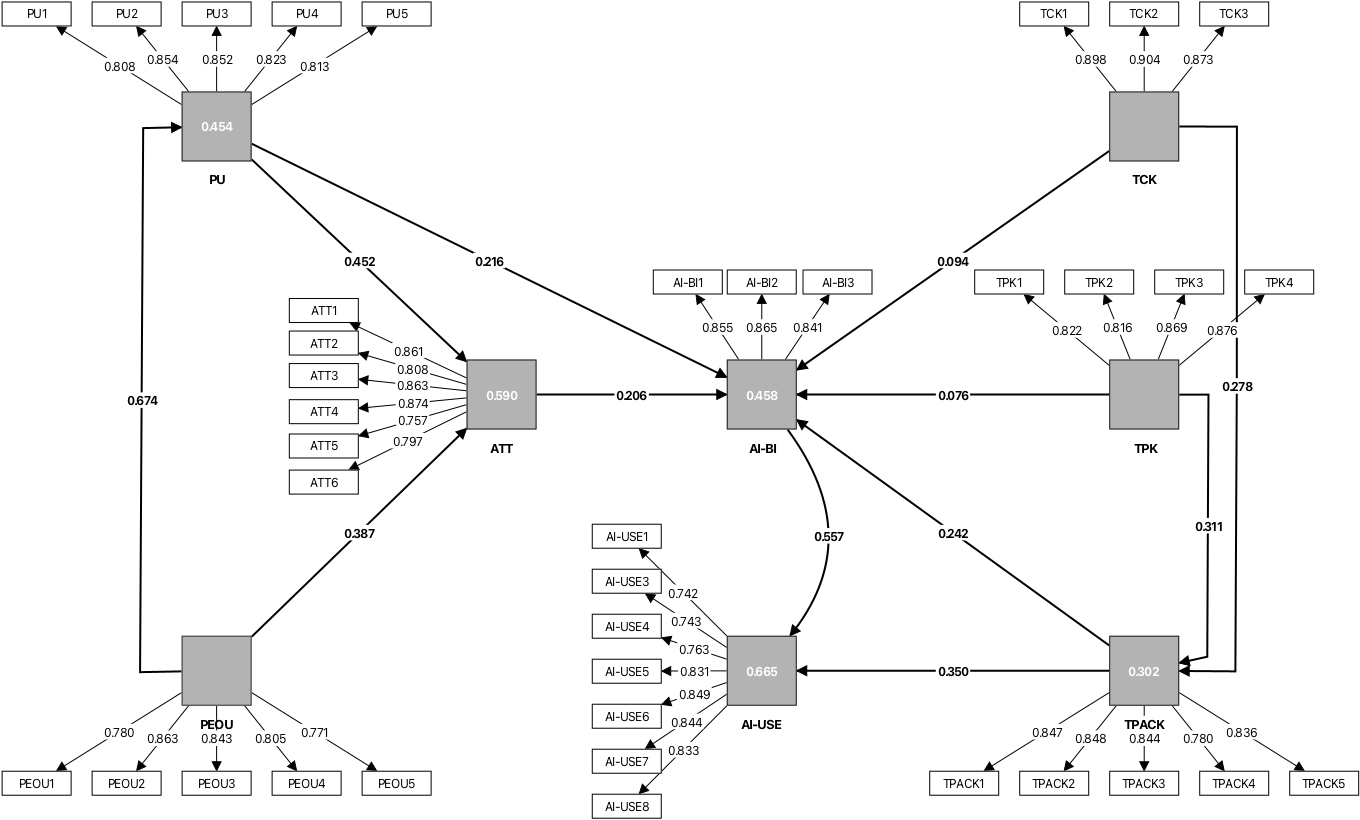
\includegraphics[width=\linewidth]{Fig2.png}
    \caption{Measurement model.}
    \label{fig2}
    \source{The authors.}
    \end{minipage}
\end{figure}

\subsection{Structural model}\label{sec-outras-estr}
We used structural model approach through SmartPLS 4.0 to report the correlations among hypothesized variables \cite{cepeda2024plssem,hair2024plssem}. \Cref{tbl5} displays the path coefficients of each proposed relationshio, t-values, and p-values, offering a thorough overview of the statistical significance. PEOU significantly influences ATT with a path coefficient of 0.387 ($\text{t-value} = 5.561$, $p < .001$) and exerts an even more significant effect on PU with a coefficient of 0.674 ($\text{t-value} = 17.887$, $p < .001$), indicating that the ease of using AI substantially affects ATT and PU. PU directly affects AI-BI with a coefficient of 0.216 ($\text{t-value }= 3.624$, $p < .001$) and ATT with 0.452 ($\text{t-value} = 7.311$, $p < .001$), underscoring the significance of perceived advantages of AI in education in shaping ATT and AI-BI. The correlation between ATT and AI-BI exhibits a path coefficient of 0.206 and a t-value of 2.841, which is statistically significant at $p < .05$, suggesting that a favorable ATT affects the intention to utilize it, albeit with a moderate effect size. TCK exerts minimal influence on AI-BI, evidenced by a path coefficient of 0.094 and a non-significant p-value of 0.103, indicating that expertise in technology within content domains may not directly correlate with utilizing AI in educational practices. TCK substantially influences TPACK with a coefficient of 0.278 ($\text{t-value} = 4.813$, $p < .001$), signifying its essential role in developing a holistic understanding encompassing pedagogy. TPACK strongly predicts AI-BI with a path coefficient of 0.242 ($\text{t-value} = 3.306$, $p < .001$) and AI-USE with 0.350 ($\text{t-value} = 8.251$, $p < .001$), underscoring its significance in both intention formation and actual AI utilization. TPK exhibits a path coefficient of 0.076 to AI-BI, which is not statistically significant ($p = 0.172$); however, it significantly influences TPACK with a coefficient of 0.311 ($\text{t-value} = 4.838$, $p < .001$), highlighting its importance in the comprehensive integration of technology into pedagogical practices. The relationship between AI-BI and AI-USE  has a path coefficient of 0.557 and a t-value of 12.848, signifying a robust positive influence of behavioral intention on actual AI use, which is statistically significant with a p-value of less than .001.

\begin{table}[h!]
\centering
\begin{threeparttable}
\caption{Structural model.}
\label{tbl5}
\begin{tabular}{llllllll}
\toprule
H & Relationship & $\beta$ & t-value & p-value & Sign. & Model fit & \\
\midrule
H1 & PEOU -\textgreater{} PU & 0.674 & 17.887 & p \textless.001 & Yes &
SRMR & 0.049  \\
H2 & PEOU -\textgreater{} ATT & 0.387 & 5.561 & p \textless.001 & Yes &
d\_ULS & 1.778  \\
H3 & PU -\textgreater{} ATT & 0.452 & 7.311 & p \textless.001 & Yes &
d\_G & 0.826  \\
H4 & PU -\textgreater{} AI-BI & 0.216 & 3.624 & p \textless.001 & Yes &
& \\
H5 & ATT -\textgreater{} AI-BI & 0.206 & 2.841 & p \textless.05 & Yes &
& \\
H6 & TCK -\textgreater{} TPACK & 0.278 & 4.813 & p \textless.00 & Yes &
& \\
H7 & TCK -\textgreater{} AI-BI & 0.094 & 1.628 & 0.103 & No & & \\
H8 & TPK -\textgreater{} TPACK & 0.311 & 4.838 & p \textless.001 & Yes &
& \\
H9 & TPK -\textgreater{} AI-BI & 0.076 & 1.366 & 0.172 & No & & \\
H10 & TPACK -\textgreater{} AI-BI & 0.242 & 3.306 & p \textless.05 & Yes
& & \\
H11 & TPACK -\textgreater{} AI-USE & 0.350 & 8.251 & p \textless.001 &
Yes & & \\
H12 & AI-BI -\textgreater{} AI-USE & 0.557 & 12.848 & p \textless.001 &
Yes & & \\
\bottomrule
\end{tabular}
\source{The authors.}
\end{threeparttable}
\end{table}

This comprehensive structural model analysis elucidates the intricate interactions among ATT, perceptions, and types of knowledge for AI use in education, presenting a refined understanding of how these elements can be utilized to improve pre-service EFL teachers’ engagement with AI technologies. The prominent pathways and their coefficients indicate areas where interventions may be most impactful, such as augmenting the PEOU of AI tools or strengthening teachers’ TPACK to promote broader AI integration in pedagogical practices. The fit indices are as follows: The SRMR is 0.049, signifying a satisfactory match, as values below 0.08 are typically deemed acceptable. The d\_ULS score is 1.778, and d\_G is 0.826; the metrics evaluate model fit in certain situations, where lower values indicate superior fit. These indices suggest that the model aligns effectively with the data, corroborating the proposed relationships in the study about AI integration in the instruction of pre-service EFL teachers \cite{magno2022pls,schuberth2023fit}.

\begin{figure}
    \centering
    \begin{minipage}{0.75\linewidth}
    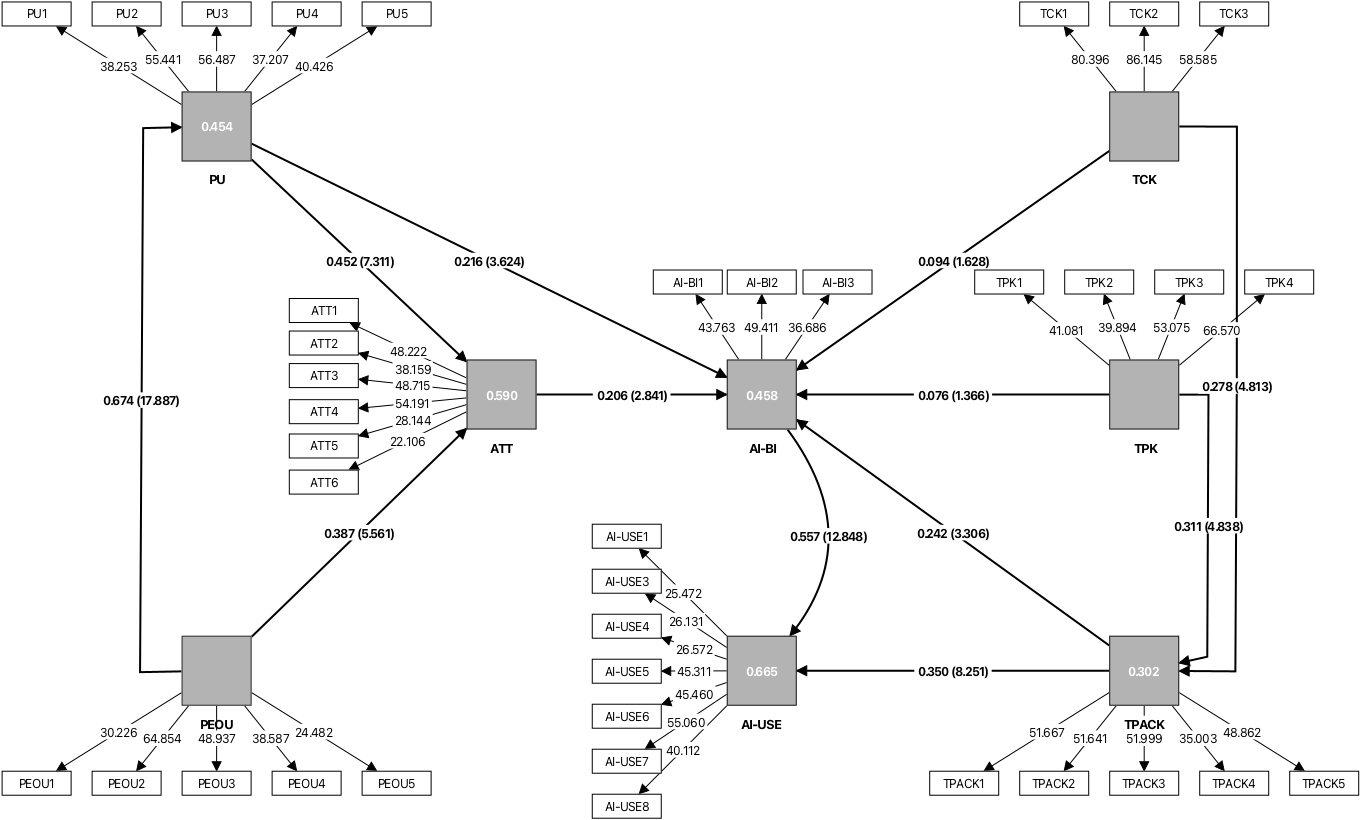
\includegraphics[width=\linewidth]{Fig3.png}
    \caption{Structural model and R\textsuperscript{2}.}
    \label{fig3}
    \source{The authors.}
    \end{minipage}
\end{figure}

\section{Discussion}\label{sec-listas}
The current study reports several factors that impact AI behavioral intention (AI-BI) and AI use (AI-USE) among Indonesian pre-service EFL teachers. PEOU significantly influences ATT and PU, with coefficients of 0.387 and 0.674, respectively, both significant at $p < 0.001$. This finding is noteworthy because it highlights the significance of usability in technology adoption, a notion reinforced by prior research from \cite{dehghani2024chatgpt}, which indicated that in educational technology, ease of use influences ATT and amplifies the perceived utility of the technology. The elevated t-values (5.561 and 17.887) a strong predictive power of PEOU for both constructs, implying that for AI to be integrated into teaching, it must be user-friendly \cite{alabdullatif2023chatbots,chen2024mr,ma2024tam,wu2023aiuse,yuviler2024chatbot}. 

PU substantially impacts AI-BI and ATT; the results align with the extensions of the TAM by \textcite{davis1989tam}, which assert that it is a pivotal factor in technology adoption, particularly in educational settings where the utility of a tool directly influences its acceptability. The strong link between PU and ATT indicates that teachers’ perseptions of AI's usefulness greatly influence how they feel about AI \cite{gumbi2024dgb,peng2022kiosks,wang2021aiadoption,weng2018tam}. ATT towards AI directly affects AI-BI although the outcome is slightly below expectations; nonetheless. The result aligns with prior reports \cite{allali2024chatgpt,dehghani2024chatgpt,ma2024tam}, who suggested that although ATT predicts behavioral intention, factors may eclipse its influence in technology adoption frameworks. The significance level indicates that a favorable disposition towards AI does influence the intention to utilize it, albeit potentially less prominently than other aspects.

TCK does not significantly affect AI-BI ($p = 0.103$), which is somewhat unexpected considering the theoretical framework suggesting that technological knowledge should forecast behavioral intents. The result contrasts the result contrasts with prior findings \cite{an2023ai,habibi2020tpack,mailizar2021tpack,sofyan2023tpack}, which indicated that subject understanding directly influences usage intentions unless accompanied by practical experience or training in the realm of swiftly advancing technology such as AI. The lack of significance may indicate a deficiency in the conceptualization or measurement of TCK for the application of AI in education, especially from pre-service EFL teachers. On the other hand, TCK has a substantial impact on TPACK, evidenced by a coefficient of 0.278 ($p < 0.05$), consistent with \textcite{mishra2009tpack} TPACK paradigm, which has been further developed by other studies \cite{an2023ai,mailizar2021tpack,sofyan2023tpack} to incorporate technologies in teaching. The significant contribution of TCK towards TPACK emphasizes that comprehending information through technological perspectives is essential for integrating AI into educational procedures. Ultimately, TPK demonstrates a substantial correlation with TPACK (0.311, $p < 0.001$) but lacks a meaningful association with AI-BI ($p = 0.172$). The computation of the data might suggest that although TPK is essential for comprehending the enhancement of education through technology, it may not directly affect the desire to utilize AI until included in a more comprehensive knowledge structure such as TPACK \cite{an2023ai,habibi2020tpack,mailizar2021tpack,mansour2024stem}. 

The substantial correlation with TPACK indicates that TPK enhances the comprehension of AI’s role in education. TPACK significantly influences AI-BI and AI-USE, supporting prior reports \cite{an2023ai,habibi2020tpack,mailizar2021tpack,mansour2024stem,sofyan2023tpack}. Teachers with a profound comprehension of the interplay between technology, pedagogy, and content are likelier to embrace and utilize AI in their instruction. The impact on AI-USE is especially significant, indicating that TPACK motivates intention and facilitates actual implementation. The association between AI-BI and AI-USE is characterized by a path coefficient of 0.557, signifying a robust and statistically significant positive correlation. This discovery corresponds with prior studies, which examined the incorporation of AI in educational environments and determined that the intention to utilize AI is a strong predictor of its actual application by educators \cite{barjestesh2025digital,baskara2024ai,lavidas2024ai,raman2023vr,strzelecki2024chatgpt,xiaohong2024intentions}. The strong t-value indicates that Indonesian pre-service EFL teachers are more likely to use AI in their instruction when they plan to use the technology.

The structured model illustrates the intricate interaction of factors affecting pre-service EFL teachers’ AI adoption. AI must be user-friendly and valuable to be successfully integrated into education, as PEOU and PU are major determinants across numerous parameters. Further research on AI knowledge structure operationalization is needed for the non-significant pathways TCK and TPK to AI-BI, suggesting that practical experience or targeted training may be required to address these issues. Technology, pedagogy, and content must be understood to increase AI adoption since TPACK affects intention and use. Our findings enhance the literature on AI in education, provide a detailed view of technology adoption patterns among potential educators, and recommend future research and policy improvements to integrate AI into teaching.

\section{Conclusion}
The current study's findings show that perceived ease of use and perceived usefulness are crucial to attitudes, AI behavioral intention, and AI use with strong coefficients. For AI to be used in education, it must be user-friendly and must be user-friendly and pedagogically beneficials. Based on the findings, educational technology must also be accessible and beneficial to boost EFL uptake. The strong links between TPACK, AI behavioral intention, and AI use present the need to combine technology experience with pedagogical and content knowledge. Technological pedagogical and content knowledge is significant, demonstrating that a thorough understanding of integrating AI into teaching techniques increases the intention to use AI in education. Non-significant paths like technological content knowledge to AI behavioral intention and technological pedagogical knowledge to AI behavioral intention suggest areas of poor comprehension or execution requiring further conceptual clarity or practical refinement. Understanding technology and its pedagogical effects is essential, but without technological pedagogical and content knowledge, it may not directly influence AI use. Practical EFL instruction that links academic understanding to real-world application may be needed. 

Given these findings, educational institutions and policymakers ought to enhance EFL teacher training programs by incorporating specialized modules on AI, highlighting usability and utility, and integrating technology with pedagogy and content. Future studies may investigate why specific knowledge components fail to directly impact AI-BI, examining whether experiential learning or targeted AI training could enhance these relationships. Furthermore, longitudinal research could evaluate the evolution of these interactions as educators accumulate experience with AI, offering a dynamic perspective on technology adoption across time. This study enhances the conversation on AI in education by providing empirical information regarding the factors that promote or obstruct AI adoption among pre-service EFL teachers. A deliberate approach to teacher education is required to convey knowledge and guarantee its practical application, cultivating a generation of educators prepared to utilize AI to improve their teaching effectiveness and student learning results.

\printbibliography\label{sec-bib}
% if the text is not in Portuguese, it might be necessary to use the code below instead to print the correct ABNT abbreviations [s.n.], [s.l.]
%\begin{portuguese}
%\printbibliography[title={Bibliography}]
%\end{portuguese}


%full list: conceptualization,datacuration,formalanalysis,funding,investigation,methodology,projadm,resources,software,supervision,validation,visualization,writing,review
\begin{contributors}[sec-contributors]
\authorcontribution{Rangga Firdaus}[conceptualization,methodology,writing]
\authorcontribution{Akhmad Habibi}[projadm,supervision,writing,review]
\authorcontribution{Robi Hendra}[methodology,formalanalysis,datacuration]
\authorcontribution{Mohd Sofian Omar Fauzee}[investigation,datacuration]
\authorcontribution{Sheren Dwi Oktaria}[visualization,review]
\authorcontribution{Muhammad Sofwan}[validation,writing]
\authorcontribution{Turki Mesfer Alqahtani}[validation,review]
\end{contributors}


\end{document}

